 \documentclass{article}

 

\usepackage{graphicx}

\newcommand{\diff}{\mathrm{d}}

\newcommand{\e}{\text{e}}

\newcommand{\im}{\text{i}}

\newcommand{\half}{\frac{1}{2}}



 

\begin{document}

\section*{Exponential - function}

 

In mathematics there are multiple famous numbers known for occuring in many interesting places in research and having various interresting properties. Examples of these are $\pi$, the imaginary unit $i$,  the golden ration $\frac{1+\sqrt{5}}{2}$ and Eulers number $e\approx2.718281828$.

 

The exponential function is then the function: $\exp(x)=e^x$. However since Euler's number is non-rational this is a somewhat weird definition mathematically sao instead the uniform convergence of it's Taylor series is often used such that the exponential function is defined as:
$$\exp(x)\equiv\sum_{i=0}^{i=\infty}\frac{x^i}{i!}$$


                             If one whishes to calculate the exponential function nummerically the Taylor series is also advantageous as it allows for the calculation of the Taylor series with arbitrary precision (or only limited by the system), by continually calculating further terms of the series.
			     Another argument for the necescity of the Taylor series is that the processor can "only" do addition, subtraction ultiplication and division, as base. So therefore taking eg $\exp(1.5)$ would be dificult as it involves squarerotts, howeever the Taylorseries does not. 
                            

                             This also leads to the implementation:

                             \begin{figure}[h]
                                                          \centering

                                                          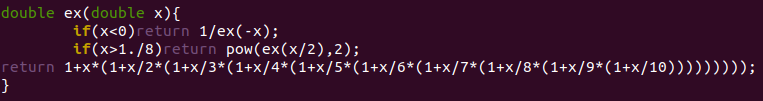
\includegraphics[width=0.65\linewidth]{code.png}

                                                          \caption{Image of an implmentaion of the exponential function using the Taylor series.}\label{fig:code}

                             \end{figure}

    This implentation starts of by checking wether or not the input is negative,
 and if it is then returns the inverse of the function value of minus the negative input (so the input is positive). 
Which is important since the precision of the sum is much better when sums are non-alternating which positive input guarantees here.

    Then the input is checked for size. The Taylor expansion is done around the point $x=0$ and so it is most accurate for values close to zero. 
So using that squaring the exponential is equivalent to doubling the input means that the input can be put arbitrarily close to zero. 
Here the Taylor series is calculated when the input reaches becomes less than $\frac{1}{8}$'th 
(notice that the input is positive by the first if statement). Finally the Taylorseries is calculated, 
this is done using a somewhat different writing method than the way it was expressed in the definition,
 this way has multiple advantages. First it advoids calling the $pow$-function which is markedly slower
 than than writing $x^*x^*x^*x...$ as is done here. Secondly it avoids calculating the factorials, in one go..
 This is good because factorials rise in value extremely quickly ($5!=120,  10!=3628800, 20!=2.4329\cdot 10^{18}$),
 which is not an issue for this implentation, but if large orders were to be calculated it becommes a good idea to avoid.
 So just to recap, first the input is made positive thoough inversion of the function-value, then the input is reduced to
 $>\frac{1}{8}$ by squaring the function-value and finally the Taylor serisees is calculated to 10'th order,
 thus giving a pretty good approximation of the exponential function.                           

                                                          \begin{figure}[h]

                                                          \centering

                                                          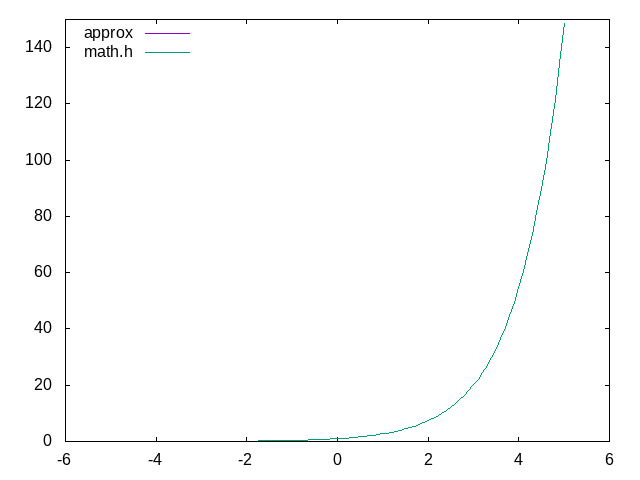
\includegraphics[width=0.65\linewidth]{exp.png}

                                                          \caption{plot of the implementation of the exponential function described above, plotted along with the implementation of the exponential function found in the package "math.h"}\label{fig:exp}

                             \end{figure}

 

                            

\end{document}	

